\chapter{Unit Tests mit Unity}
\label{chap:Unit Tests mit Unity}

Da Tests ein essentieller Teil der testgetriebenen Entwicklung sind, ist das Test-Framework ein wichtiger Bestandteil für ein Projekt. Für Unity gibt es keine offizielle Testumgebung, allerdings wurden von der Community welche entwickelt.

Im nachfolgenden Kapitel werden die in Frage kommenden Frameworks vorgestellt und verglichen. Anschließend erläutern wir unsere Entscheidung für das gewählte Framework.

\section{Unit Test Framework der Entwicklungsumgebung (MSTest)}

Das Nächstliegende ist es, das Framework der Entwicklungsumgebung zu verwenden. Dies wäre in diesem Fall MSTest, welches in Visual Studio integriert ist.\\
Hierbei ist es üblich, dass man neben dem Projekt mit dem Produktivcode ein weiteres für die Tests hat. Dadurch sind diese und das Produkt sowohl räumlich, als auch logisch voneinander getrennt. Am einfachsten erstellt man dieses Testprojekt mit Hilfe einer Vorlage von Visual Studio, in dem die benötigten Referenzen - die Bibliothek des Test Frameworks - schon vorhanden sind. Die Vorlage befindet sich im Reiter \textit{Test} und heißt \textit{Komponententestprojekt} beziehungsweise \textit{Unit Test Project}.\\
Alternativ kann man die benötigte Bibliothek auch manuell als Referenz hinzufügen. Diese findet man in \textit{Assemblies -> Extension} unter dem Namen \textit{Microsoft.VisualStudio. QualityTools.UnitTestFramework}. Als weitere Referenz muss man das Projekt des zu testenden Produkts hinzufügen, um Zugriff auf die darin enthaltenen Klassen zu bekommen.

Im Nachfolgenden wird gezeigt, wie man einen Unit-Test mit MSTest aufbaut und welche Möglichkeiten es dabei gibt.

\pagebreak
\begin{lstlisting}[caption={[Unit Test mit MSTest]Unit Test mit MSTest\\
Beispiel einer Testklasse in MSTest. Zeigt wie man ihre Testmethoden deklariert und wie sie initialisiert wird.}, label=code:UnitTestMitMSTest]
using Microsoft.VisualStudio.TestTools.UnitTesting;

namespace Test_Project {
	[TestClass]
	public class UnitTest {
		[ClassInitialize]
		public static void ClassSetUp() {
			// Code to initialize the test class
			// Is called only once BEFORE all tests
		}
		[TestInitialize]
		public void SetUp() {
			// Code to intialize the single tests
			// Is called BEFORE every test
		}
		[TestMethod]
		public void TestSomething() {
			// A test
		}			
		[TestMethod]
		public void TestSomethingOther() {
			// An other test
		}
		[TestCleanup]
		public void TearDown() {
			// Code to clean the actions of the single tests
			// Is called AFTER every test
		}
		[ClassCleanup]
		public static void ClassTearDown() {
			// Code to clean the test class
			// Is called only once AFTER all tests
		}
	}
}
\end{lstlisting}
\pagebreak

Um dem Framework zu signalisieren, dass in einer Klasse Tests vorhanden sind, braucht diese das Attribut \textit{TestClass}, welches in eckigen Klammern über dem Klassennamen angegeben wird. Die einzelnen Tests in Form von Methoden werden durch \textit{TestMethod} gekennzeichnet und dürfen nichts zurückgeben und keine Parameter erwarten. Innerhalb dieser Methoden kann man mit Hilfe der Klasse \textit{Assert} bestimmte Bedingungen festlegen, die erfüllt sein müssen. Sind sie es nicht, schlägt der Test fehl und es wird eine entsprechende Meldung angezeigt. Auch wenn eine Exception nicht gefangen wird, schlägt der Test fehl und zeigt die Nachricht der Exception an.\\
Außerdem können bestimmte Methoden vor den einzelnen Tests ausgeführt werden, um zum Beispiel benötigte Objekte zu initialisieren. Dabei unterscheidet man zwischen einem Klasseninitialisierer, der genau einmal vor dem Aufruf der ersten Testmethoden ausgeführt wird und dem Testinitialisierer, der vor jedem Aufruf einer Testmethode durchgeführt wird. Der Klasseninitialisierer muss statisch sein und wird durch das Attribut \textit{ClassInitialize} markiert. Er kann zum Beispiel genutzt werden, um eine Verbindung zu einer Datenbank aufzubauen, die von mehreren Testmethoden der Testklasse verwendet wird. Der Testinitialisierer muss mit \textit{TestInitialize} gekennzeichnet werden und könnte zum Beispiel Objekte initialisieren, die von mehreren Tests gebraucht und verändert werden. Da diese dadurch vor jedem Test neu initialisiert werden, bleiben die Tests unabhängig voneinander.\\
Entsprechend zu den Initialisierern kann man auch spezielle Methoden definieren, die nach den Tests ausgeführt werden sollen. Der Klassenbereiniger könnte die zuvor geöffnete Verbindung mit der Datenbank schließen und diese von etwaigen Testdaten befreien. Der Testbereiniger kann zum Beispiel verwendet werden, um eine Singleton-Klasse auf ihren Ursprungszustand zurückzusetzen, falls dies notwendig sein sollte.

Um die Tests auszuführen geht man in der Menüleiste von Visual Studio 2012 auf \textit{Test} und wählt \textit{Run -> All Tests}. Daraufhin sucht Visual Studio alle Testklassen in der Solution, führt diese aus und listet das Ergebnis auf. Dies kann man in \autoref{fig:VisualStudioTestExplorer} sehen.

Detailliertere Informationen über das Unit Test Framework von Microsoft erhält man auf deren MSDN-Bibliotheksseite unter \url{http://msdn.microsoft.com/de-de/library/dd264975.aspx}.

Allerdings gibt es schwerwiegende Probleme, wenn man mit MSTest ein Unity-Skript testen möchte, worauf in \textit{\autoref{sec:Vergleich_und_Entscheidung} \nameref{sec:Vergleich_und_Entscheidung}} näher eingegangen wird.

\section{UUnit}

UUnit\footnote{Weitere Informationen unter \url{http://wiki.unity3d.com/index.php?title=UUnit}} ist ein Projekt der Fangemeinde für ein rudimentäres Unit Test Framework, welches in Unity Projekten verwendet werden kann. Es wurde zunächst in \textit{Boo} geschrieben, wodurch es auch Tests in \textit{Boo} erwartet. In der neusten Version (Veröffentlicht am 21.08.2012) wurde es allerdings nach C\# portiert.
Um mit UUnit Tests ausführen zu können, muss man das Framework in sein Projekt einbinden. Da UUnit Open-Source ist kann man das gesamte Framework innerhalb des \textit{Assets}-Ordners ablegen. Alternativ könnte man das Framework auch zu einer Bibliothek kompilieren und diese als Referenz einbinden.

Testklassen von UUnit müssen von der Klasse \textit{UUnitTestCase} erben, welche die beiden virtuellen Methoden \textit{SetUp} und \textit{TearDown} zur Verfügung stellt. Diese werden vor beziehungsweise nach jeder Testmethode durchgeführt und können von den expliziten Tests überschrieben werden.\\
Die Testmethoden werden durch das Attribut \textit{UUnitTest} gekennzeichnet und mit der Klasse \textit{UUnitAssert} können Bedingungen definiert werden, die den Test fehlschlagen lassen, sollten sie nicht erfüllt sein. Allerdings bietet diese nur sechs Arten von Bedingungen, wozu \textit{Fail}, \textit{True} und \textit{Equals} gehören. Eine \textit{NotEquals}-Bedingung gibt es zum Beispiel nicht.

Innerhalb von UUnit gibt es die Klasse \textit{UUnitTestRunner}, welche alle Tests innerhalb des Projekts ausführt und das Ergebnis ausgibt. Kopiert man die Quelldatei dieser Klasse in den Ordner \textit{Assets/Standard Assets/Editor} des Unity-Proejkt, wird sogar ein neuer Knopf in die Menüleiste der Unity SDK hinzugefügt, mit dem man alle Tests ausführen lassen kann. Möchte man die Datei nicht zu seinem Projekt hinzufügen, kann man auch folgendes Skript schreiben und einem beliebigen \textit{GameObject} anfügen.
\pagebreak

\begin{lstlisting}[caption={[Beispiel um alle UUnit-Tests auszuführen]Beispiel um alle UUnit-Tests auszuführen\\
Muss an ein \textit{GameObject} angehängt werden. Beim Start des Spiels werden alle Tests ausgeführt.}, label=code:UUnitTestRunner]
public class TestRunner : MonoBehaviour {
	public void Start() {
		UUnitTestRunner runner = new UUnitTestRunner();
		runner.RunAllTests();
	}
}
\end{lstlisting}

Die Ergebnisse des Testdurchlaufs werden auf der Konsole von Unity ausgegeben, was man in der Abbildung unten sehen kann. Dabei werden die Fehlermeldungen der fehlgeschlagenen Tests, sowie die Anzahl der durchgeführten und fehlerhaften Tests ausgegeben.

\begin{figure}[h]
\centering
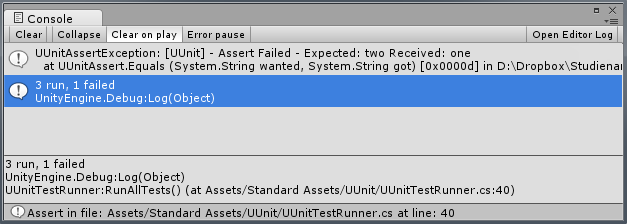
\includegraphics[width=1\linewidth]{./images/Kapitel_UnitTestsMitUnity/UUnit_Konsolenausgabe}
\caption[Ausgabe von UUnit]{Ausgabe von UUnit}
\label{fig:UUnit_Konsolenausgabe}
\end{figure}
\clearpage

\section{SharpUnit}\label{sec:SharpUnit}

SharpUnit\footnote{Weitere Informationen unter \url{http://wiki.unity3d.com/index.php?title=SharpUnit}} ist auch ein Projekt der Fangemeinde und ist in C\# implementiert. Es wurde entwickelt, da UUnit zunächst nur in \textit{Boo} zur Verfügung stand. Es orientiert sich an UUnit und hat einige Gemeinsamkeiten damit.\\
Um Tests ausführen zu können, muss man SharpUnit in sein Unity-Projekt einbinden, was wie mit UUnit funktioniert.

Testklassen müssen bei SharpUnit von der Klasse \textit{TestCase} erben, welche es ermöglicht die Methoden \textit{SetUp} und \textit{TearDown} zu überschreiben. Testmethoden werden durch das Attribut \textit{UnitTest} gekennzeichnet. Auch SharpUnit stellt einem eine Klasse zur Definition von Bedingungen zur Verfügung, wobei diese in etwa denen von UUnit entsprechen. Allerdings fehlt \textit{Fail} mit dem man einen Test geziehlt fehlschlagen lassen kann. Dafür gibt es die Möglichkeit, eine erwartete Exception zu definieren. Dies beschränkt sich allerdings auf eine pro Test, das heißt man kann keine zwei Exceptions innerhalb einer Testmethode erwarten.
 
Im Gegensatz zu UUnit können die Tests von SharpUnit nur zu Beginn des Spiels ausgeführt werden. Dafür benötigt man ein Skript, welches in der \textit{Start}-Methode bestimmte Aktionen ausführt und an ein \textit{GameObject} angehängt wird. Der nachfolgende Code ist das Beispiel von SharpUnit für so ein Skript.
\pagebreak

\begin{lstlisting}[caption={[Einbindung der Tests mit SharpUnit]Einbindung der Tests mit SharpUnit\\
Quelle: Demo von SharpUnit, erhältlich unter \url{https://github.com/mgants4/SharpUnit}.}, label=code:SharpUnitTestRunner]
public class Unity3D_TestRunner : MonoBehaviour {
	void Start() {
        // Create test suite
        TestSuite suite = new TestSuite();

        // Example: Add tests to suite
        suite.AddAll(new Dummy_Test());

        // Run the tests
        TestResult res = suite.Run(null);

        // Report results
        Unity3D_TestReporter reporter = new Unity3D_TestReporter();
        reporter.LogResults(res);
	}
}
\end{lstlisting}

Zunächst wird eine SharpUnit \textit{TestSuite} erzeugt, zu der die zu testenden Tests hinzugefügt werden. Dafür ruft man \textit{AddAll} der Suite auf und übergibt ihr eine Instanz einer Testklasse, wodurch deren Testmethoden registriert werden. Hat man die gewünschten Tests hinzugefügt, ruft man \textit{Run} der Suite auf. Diese führt die registrierten Tests aus und gibt einem Informationen über den Verlauf, in Form einer Instanz von \textit{TestResult}, zurück. Im letzten Schritt muss man einen Test-Reporter erzeugen, um damit das Ergebnis auf der Konsole der Unity SDK auszugeben. Die Ausgabe ist sehr ähnlich mit der von UUnit, zu sehen in \autoref{fig:UUnit_Konsolenausgabe}.
\pagebreak

\section{Vergleich und Entscheidung}\label{sec:Vergleich_und_Entscheidung}

In diesem Abschnitt wird die Tauglichkeit für die testgetriebene Entwicklung mit den unterschiedlichen Unit-Test-Frameworks verglichen und wir erläutern unsere Entscheidung, mit welchem wir den Prototypen implementieren wollen.

\paragraph{MSTest} Die Vorteile des von Microsoft mitgelieferten Test-Frameworks sind zahlreich. Es hat die beste \textit{Assert}-Klasse um die Bedingungen der Tests zu formulieren, da sie viele Methoden bietet. Außerdem stellt es einem als einziges die Möglichkeit zur Verfügung, einen Klasseninitialisierer/reiniger zu definieren.\\
Die Tests müssen von keiner anderen Klasse erben, sondern werden lediglich durch ein Attribut markiert. Außerdem hat man nur wenig Aufwand, um die Tests auszuführen. Das Ergebnis des Durchgangs wird nicht in der Konsole ausgegeben, sondern als Liste der einzelnen Testmethoden. Diese Liste wird in erfolgreiche, fehlgeschlagene und nicht ausgeführte Tests unterteilt. Verwendet man das Plugin \textit{Resharper} werden die Ergebnisse mit einem Baum angezeigt, was noch übersichtlicher ist.\\
Dadurch, dass MSTest unabhängig von Unity ist, sind auch die Tests unabhängig von dem Projekt. Im Gegensatz zu den anderen Frameworks, müssen sich die Tests nicht innerhalb des Unity-Projekts befinden, sondern liegen in einem separaten Projekt.

Es gibt allerdings auch Nachteile. Zum Beispiel kann die Ergebnisliste bei vielen Tests unübersichtlich werden und das Ausführen aller Tests dauert beim ersten mal ungewöhnlich lange. Diese Probleme kann man mit der Verwendung von \textit{Resharper} beseitigen.\\
Ein äußerst schwerwiegendes Problem ist allerdings, dass man mit MSTest keine Skripte - genauer gesagt keine Klassen die von \textit{MonoBehaviour} erben - testen kann. Wenn man in einem Test ein Skript erzeugen möchte, tritt eine \textit{SecurityException} auf, die den Test fehlschlagen lässt. Dies liegt daran, dass die Klasse \textit{MonoBehaviour} nur in einer laufenden Unity-Umgebung intialisiert werden kann. Diese lässt sich nicht in einem Test initialisieren oder simulieren. Als Folge müsste man die Logik des Spiels soweit es geht aus den Skripten herausziehen, um eine ausreichende Testabdeckung zu erhalten.

\paragraph{UUnit und SharpUnit} Da sich diese beiden Frameworks sehr ähnlich sind, werden sie zusammen betrachtet. Der Vorteil ist, dass man Skripte automatisiert testen kann, da die Frameworks in der Unity SDK laufen. Diese Funktionalität wurde unterschiedlich gut umgesetzt. So kann man nur mit UUnit die Tests ausführen, ohne dass ein \textit{GameObject} und ein Skript benötigt wird. Dabei werden allerdings zwingend alle Tests des Projekts ausgeführt.

Nachteile sind vor allem die spärlichen Methoden der \textit{Assert}-Klassen und dass die Ausgabe über die Konsole erfolgt, was sehr unübersichtlich werden kann. Außerdem kann man nicht direkt von den Ergebnissen zu der Quelldatei des Tests springen.\\
Möchte man nur bestimmte Tests ausführen, benötigt man jedenfalls ein Skript, in dem man die ausgewählten Tests hinzufügen muss, sowie ein \textit{GameObject} an welches man das Skript anhängt. Bei SharpUnit muss man zusätzlich noch ein Objekt erzeugen, um das Testergebnis auszugeben.\\
Weiterhin sind die Tests nun ein Teil des Unity-Projekts, was man bei der finalen Versionen beachten sollte, damit die Testklassen und Testszenen nicht mit ausgeliefert werden.\\
Ein weiteres großes Problem ist, dass die Tests nur zu Beginn des Spiels ausgeführt werden können, da man sie üblicherweise in der \textit{Start}-Methode eines Skripts aufruft. Da es keine Möglichkeit gibt den Tests einen Zeitpunkt zuzuordnen, zu dem sie ausgeführt werden sollen, macht eine Verlagerung in die \textit{Update}-Methode keinen Sinn. Außer man entwickelt dafür eine eigene Logik, was allerdings nicht trivial ist. Stattdessen würde das Verlagern in die \textit{Update}-Methode zur Folge haben, dass die Tests bei jeder Berechnung eines Frames durchgeführt werden.\\ Mit den Frameworks kann man zwar testen, dass die Skripte korrekt erstellt werden, ihre Methoden funktionieren und man ihre Attribute nicht mit unerlaubten Werten füllt. Allerdings sind Integrations- und Akzeptanztests in einem laufenden Spiel nicht möglich. Somit lässt sich kein richtiges End-to-End Testen realisieren, was wichtig für die testgetriebene Entwicklung ist.

Aufgrund der oben aufgeführten Nachteile von SharpUnit und UUnit, halten wir es für wenig sinnvoll diese zu verwenden. Denn die Hauptaufgabe eines Skripts sollte die Interaktion mit der Spielwelt sein. Da man diese nicht ohne einen erheblichen Mehraufwand testen kann, haben wir uns dazu entschieden, ausschließlich MSTest zu verwenden. Dadurch müssen wir die Spiellogik aus den Skripten auslagern, um diese testen zu können.

Als Zwischenfazit kann man bereits angeben, dass ein wie oben beschriebener Ablauf von TDD nicht möglich ist. Wir möchten dennoch herausfinden, ob und welche Vorteile sich aus einer großen Testabdeckung ergeben. Daher werden wir soweit wie möglich testgetrieben entwickeln.